         
\section{The Algorithm}
\label{informal-specification}

In  this  section   we  informally  describe the   garbage  collection
algorithm.   As illustrated  in    Figure~\ref{gc-figure}, the  system
consists of two processes, the  {\em mutator} and the {\em collector},
working on a shared {\em memory}.

\begin{figure}[htb]
\center
%\makebox[\textwidth]{\epsfbox{gc-fig.ps}}
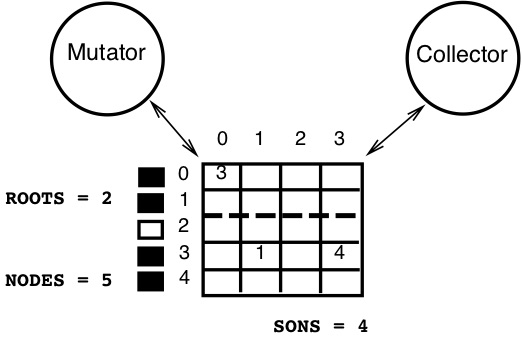
\includegraphics[width=2.5in]{gc-fig.jpeg}
\caption{The Mutator, Collector and Shared Memory}
\label{gc-figure}
\end{figure}

\subsection{The Memory}

The memory is a fixed size array of  {\em nodes}.  In
Figure~\ref{gc-figure} there 
are 5 nodes (rows) numbered 0--4.  Associated with  each node is an
array of uniform  length of {\em cells}.     Figure~\ref{gc-figure} shows
4 cells numbered 0 -- 3 per node.  A cell is  identified by a pair
of  integers ($n$,$i$) where  $n$ is  a node number  and where  $i$ is
called   the {\em index}.   Each  cell  contains a pointer   to a node,
called the {\em son}.  In the case   of a LISP  implementation, there  are, for
example, two  cells per node.  In   Figure~\ref{gc-figure}, we  assume
that all empty 
cells contain  the  {\em NIL} value 0,   and hence point to   node 0.  In
addition, node 0 points to node 3 (because  cell (0,0) does so), which
in turn points to nodes 1 and  4.  Hence the memory  can be thought of
as a two-dimensional  array, the  size of  which is  determined by the
positive integer constants  {\tt NODES} and {\tt  SONS}\@.   Each node
has an  associated  {\em colour},  black or white,  that  is used by the
collector in identifying garbage nodes.

A pre-determined number of   nodes, defined  by the positive   integer
constant {\tt  ROOTS}, are designated  as the  {\em roots},  and these are
kept in the initial  part  of the array (they   may be thought of   as
static program variables).   In  Figure~\ref{gc-figure}, there  are two
such  roots shown separated from the rest with a dotted line. A node is {\em
accessible} 
if it can be reached from a root by  following pointers, and a node is
{\em garbage} if it is not accessible. Nodes 0, 1, 3, and 
4  in Figure~\ref{gc-figure} are therefore accessible, and node 2 is
garbage. 

\noindent There  are  only three operations by which
the memory structure can be modified:

\begin{itemize}
  \item Redirect a pointer towards an accessible node.
  \item Change the colour of a node.
  \item Append a garbage node to the free list.
\end{itemize}

\noindent In the initial state, all pointers are assumed to  be 0, 
and nothing is assumed about the colours.


\subsection{The Mutator}

The mutator  corresponds to  the user  program  and performs the  main
computation.  From an abstract point of  view, it continuously changes
pointers  in the memory; the   changes being arbitrary except for  the
fact that  a cell can  only be set to point  to an  already accessible
node. In  changing a  pointer  the ``previously pointed-to'' node  may
become garbage,  if it  is  not accessible   from  the roots  in  some
alternative way.  In  Figure~\ref{gc-figure}, any cell can hence be
modified by the 
mutator to point to a node other than  2.  Only
accessible  cells can be modified, but as shown below,  the algorithm can
in fact be proved safe  without this restriction.  The algorithm is as
follows: 
\begin{enumerate}

\item Select a node $n$, an index $i$, and an accessible node $k$,
      and assign $k$ to cell ($n$,$i$). 
      
\item Colour node $k$ black. Return to step 1.

\end{enumerate}

\noindent Each of the two steps is regarded as an atomic instruction.


\subsection{The Collector}

The collector collects  garbage nodes and  puts
them into  a {\em free list}, from  which the  mutator may then remove
them as they are needed during dynamic storage allocation.  Associated
with each node is a {\em colour} field, that is used  by the collector
during  its  identification of garbage  nodes.  Basically,  it colours
accessible nodes {\em  black}, and at  a certain point it collects all
{\em white} nodes, which are then garbage, and puts them into the free
list. Figure~\ref{gc-figure} illustrates the situation at such a  point:
only node  2 is white since  it is the only garbage node.  The collector
algorithm is as follows:
%
\label{the-collector-informal}
\begin{enumerate}

\item Colour each root black.

\item Examine each pointer in succession. If the source is black and the
      target is white, colour the target black.

\item Count the black nodes. If the result exceeds the previous count (or
      if there was no previous count), return to step 2.

\item Examine each node in succession. If a node is white, append it to
      the free list; if it is black, colour it white. Then return to step 1.

\end{enumerate}

Steps 1--3 constitute the {\em marking}  phase where 
all accessible   nodes are blackened.  Each of these steps involves an
iteration involving a smaller step that is executed atomically.  
For example,  step~3
consists   of several atomic instructions,  each  counting (or not) a
single node.


%%% Local Variables: 
%%% mode: latex
%%% TeX-master: t
%%% End: 
